% 20200719
\documentclass[../thesis.tex]{subfiles} %% use packages & commands as this main file
\begin{document}
\section{Result}
Numerical simulation showed stability in biomass densities on destructive harvest systems for both \PoN\ and \PBN\ (Fig.\ref{f:destCarbon}).  After an initial boost of organic carbon accumulation (Fig.\ref{f:destCarbon}A), \phy-only systems had linear accumulation of organic carbon but \pbs\ had its level slightly dropped to a stable level and perpetuated.  The difference in carbon accumulation trend led to non-significant different between \PoN\ systems only after a few days of system establishment (Fig.\ref{f:ydDaily}A \& \ref{f:ydByHarv}A).  We did not observe this pattern in \pbs.

Pairwise Wilcox test showed statistical significance for all four systems (\PBH, \PoH, \PBN\ \& \PoN).  Yet in Fig.\ref{f:ydByPara} the pair of \phy-only systems were largely overlapping and the overlap was also observed for the \pbs s.  Hence we concluded that biological significance was only between \phy-only and \pbs s but not across harvest terms within each pair.

Biological parameters for \phy\ (Fig.\ref{f:ydByPara}A-D) had stable influence over \phy-only systems (\PoH\ \& \PoN) in the view of the median.  No parameters had influence on median values for \pbs s (\PBH\ \& \PBN\ in Fig.\ref{f:ydByPara}A-H).  As for \phy\ biological parameters, only intraspecific interference ($\aP$) had a decreasing effect in a decreasing rate.  Hence density-insensitive \phy\ death rate had much higher productivity than others; maximum yield for all four systems concentrated at the minimal value for this parameter range.  The other three \phy\ parameters (i.e. non-respirable carbon fraction for \phy\ $\ePR$, carbon fraction allocated into biomass for \phy\ $\eP$ and \phy\ growth rate $\gP$) had a stable positive influence on median of \phy-only systems yield fluxes.  Although pairwise Wilcox test showed significance (p $\ll$ 0.01) between \PoH\ and \PoN, the difference may not be biological significant.  The set of four parameters had no observational effect on \pbs s.  The reason was because most of the raw yield from simulations were zeros.  Details were listed later in this section.

Biological parameters for \bac\ (Fig.\ref{f:ydByPara}E-H) had no observable influence over all systems.  Since these four parameters had no mathematical effect on \phy-only systems (equilibrium 3 in Table \ref{t:eqm}), fluctuations from \phy-only systems in Fig.\ref{f:ydByPara}E-H was due to LHS sampling effect.  Yet, it also had no observational effect on \pbs s, probably because of the large number of zero yield scenarios.

Log distributions for \phy-only systems were stable with much wider yield ranges than \pbs\ regardless of harvest mode (Fig.\ref{f:ydByHarv}B).  On a contrary, most \PBH\ systems yielded 0 \dxdt\ (for both medians and interquartile ranges).  \PBN\ systems however had both positive and negative yields (median -0.00001, IQR [-0.00025 - +0.00106]\dxdt) depending on the systems' perpetuation time.  For maximum yield scenarios of each of the four systems, \PoH\ and \PoN\ had similar yields of 345\dxdt ($T$ = 19900 for \PoN; $x$ = 19501 for \PoH).  Maximum yield for \PBH\ systems was 285 ($x$ = 2101) \dxdt\ and that for \PBN\ systems was 243 ($T$ = 90) \dxdt.  The set of phytoplankton features was similar across all four systems (Fig.\ref{f:ydByPara}A-D).  Maximum yield systems preferred high carbon to biomass conversion efficiency (both $e_{PR}$ \& $e_P$ high values) under moderate-high growth rate and minimal population density sensitivity.  Although bacteria only appeared in \pbs s, requirements for maximum yield were different between \PBN\ and \PBH\ (Fig.\ref{f:ydByPara}E-H).  A \PBN\ system required high leakage bacteria (high $e_{BR}$ \& low $e_B$) with very high growth rate and high death rate.  On the other hand, \PBH\ systems needed a balanced carbon to biomass level (moderate $e_{BR}$ \& moderate $e_B$).  High growth and low death rates favoured yield accumulation.  In short, all four systems had similar preferences on phytoplankton.  But if \bac\ was involved, requirement for the best \bac\ was strict and specific based on the designated type of system.

Among the four system sets within the LHS scenarios (1.1 million), feasible (for continuous harvest systems) and favourable (for destructive harvest systems) were counted.  Feasible systems were systems that a biological meaningful carbon density at the stable state of such system were analytically calculated.  For \PoH, 88.3\% (n=971039) were feasible.  On a contrary, only 0.3\% (n=3251) of \PBH\ systems were feasible.  Favourable systems were scenarios that had a net gain of carbon during numerical integration.  99.5\% (n=1094500) \PoN\ systems but 47.0\% (n=517113) \PBN\ systems were favourable.  Compare the number of feasible/favourable systems with the maximum yield (Fig.\ref{f:ydByPara}), it showed \phy-only systems were easy to construct with high yield.  Yet a fit \bac\ candidate could also bring carbon harvest up to high levels.

\begin{figure}[H]
    \centering
    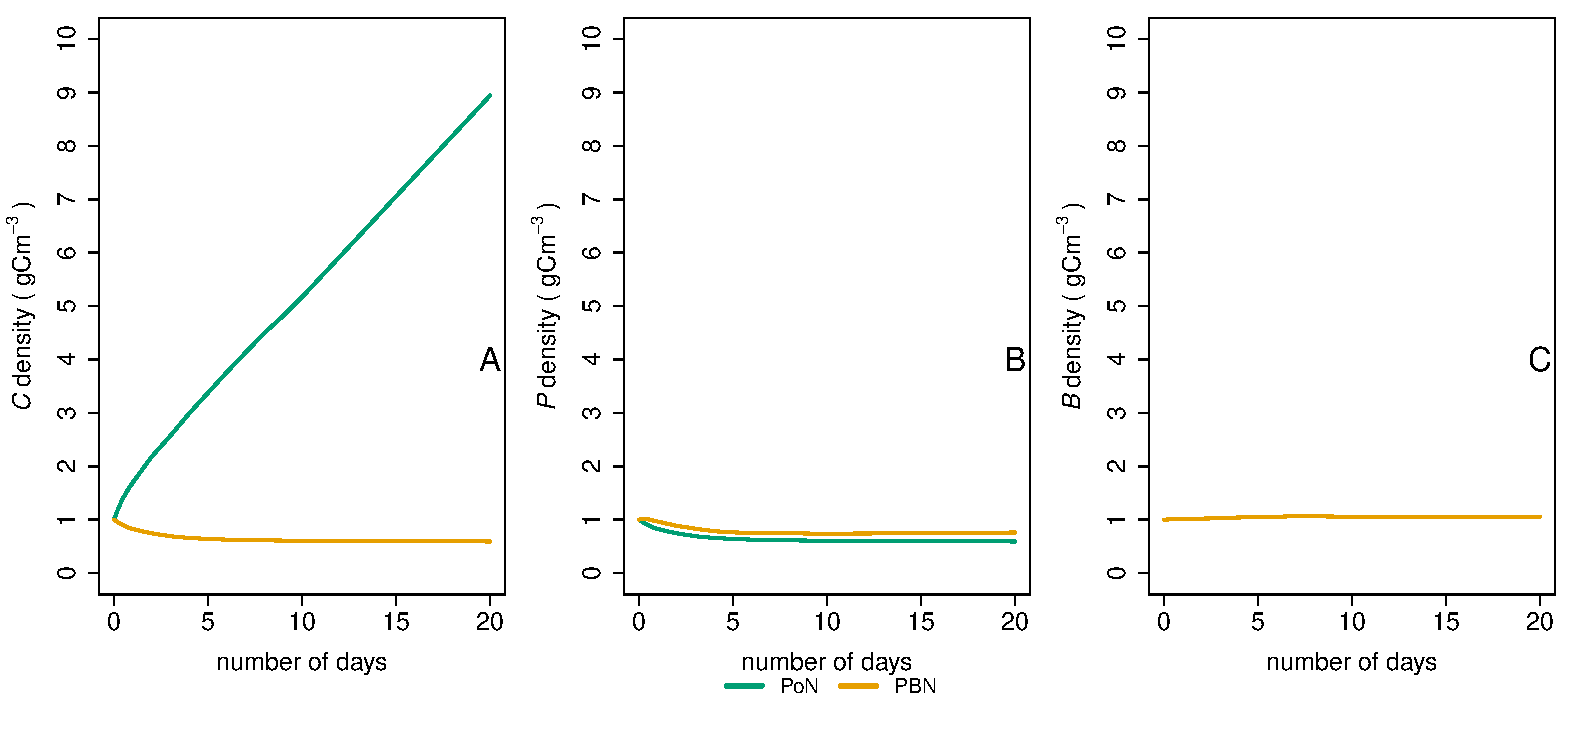
\includegraphics[width=\linewidth]{result/Sample.pdf}
    \caption[Median carbon content in destructive systems]{Median carbon content in destructive systems.  $C$, $P$ and $B$ were carbon pools in Fig.\ref{f:model}.  Eq.\ref{eq:PBH} was used with different initial carbon densities to address the \PoN\ and \PBN\ modes.  Initial carbon densities for \PoN\ were [1,1,0]\den\ ($C$, $P$, $B$) and that for \PBN\ were [1,1,1]\den.  Note that both systems had similar levels of \phy\ across time \textbf{(B)}.  Yet due to the presence of \bac\ \textbf{(C)}, organic carbon pool density changes were huge \textbf{(A)}.  Also note that after a initial boost, accumulation of organic carbon was linear for \PoN\ \textbf{(A)}.  Note that existence of \bac\ suppressed the organic carbon density in the system \textbf{(A)} with almost unchanged \bac\ biomass density \textbf{(C)}.}
    \label{f:destCarbon}
\end{figure}

\begin{figure}[H]
    \centering
    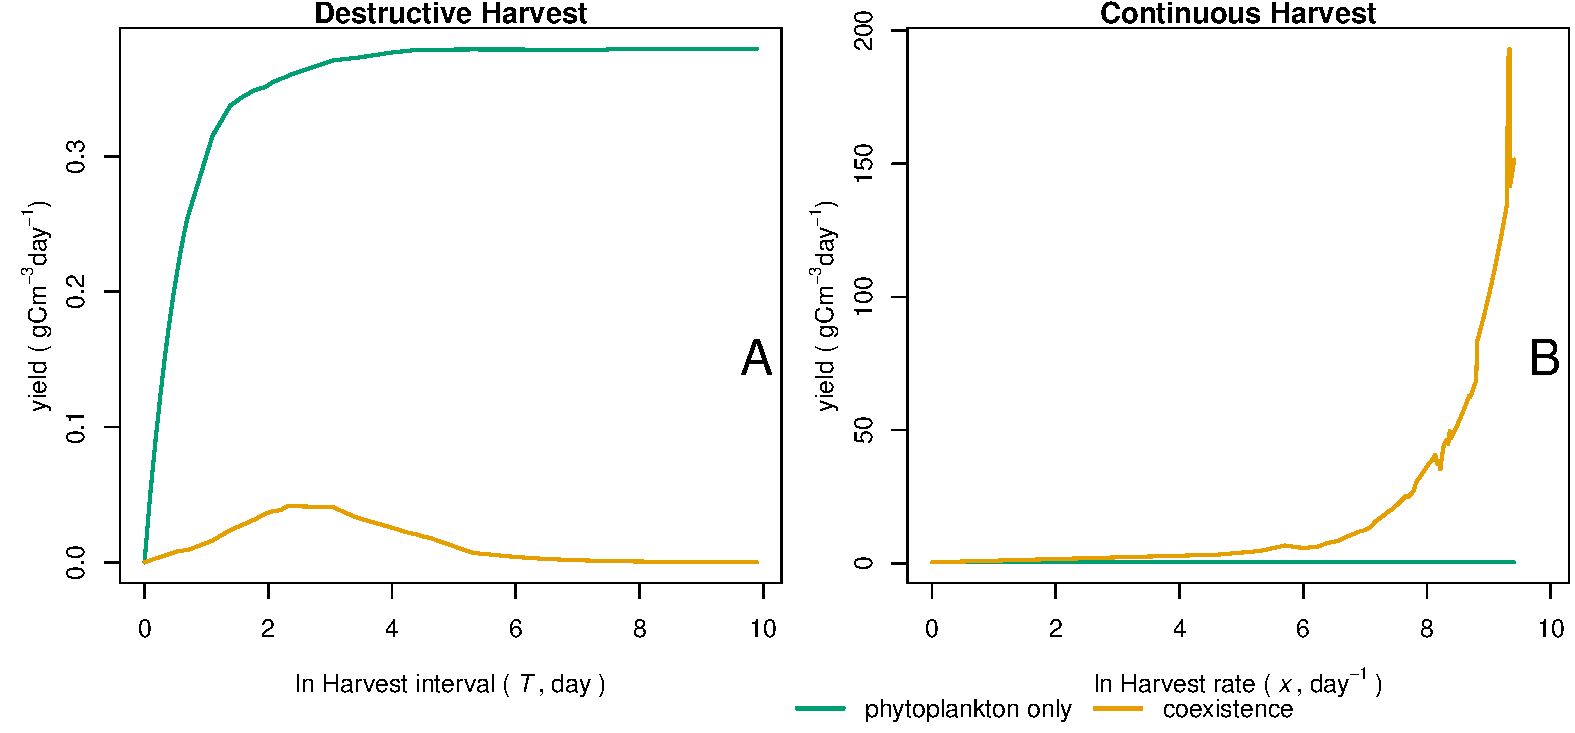
\includegraphics[width=\linewidth]{result/DailyYield.pdf}
    \caption[Median daily yield across systems]{Median daily yield across systems.  Note that both harvest interval/rate were natural logged to emphasize daily yield changes when carbon was harvested more frequent \textbf{(A)} or less amount \textbf{(B)}.  Also note that lower part of \textbf{(B)} was empty because we did not collect such fine-scaled data.  In plot \textbf{A}, the minimal optimum harvest interval for \PoN\ was around 55 days (i.e. exp(4)) while peak yield achieved at day 20 (i.e. exp(3)) for \PBN.  For continuous harvest \textbf{(B)}, very high daily harvest destabilised \PoH\ systems.  Yet for majority of \PBH\ systems, daily yield was zero because such system only feasible for a tiny portion (0.3\%) of the 1.1 million simulated scenarios.}
    \label{f:ydDaily}
\end{figure}

\begin{figure}[H]
    \centering
    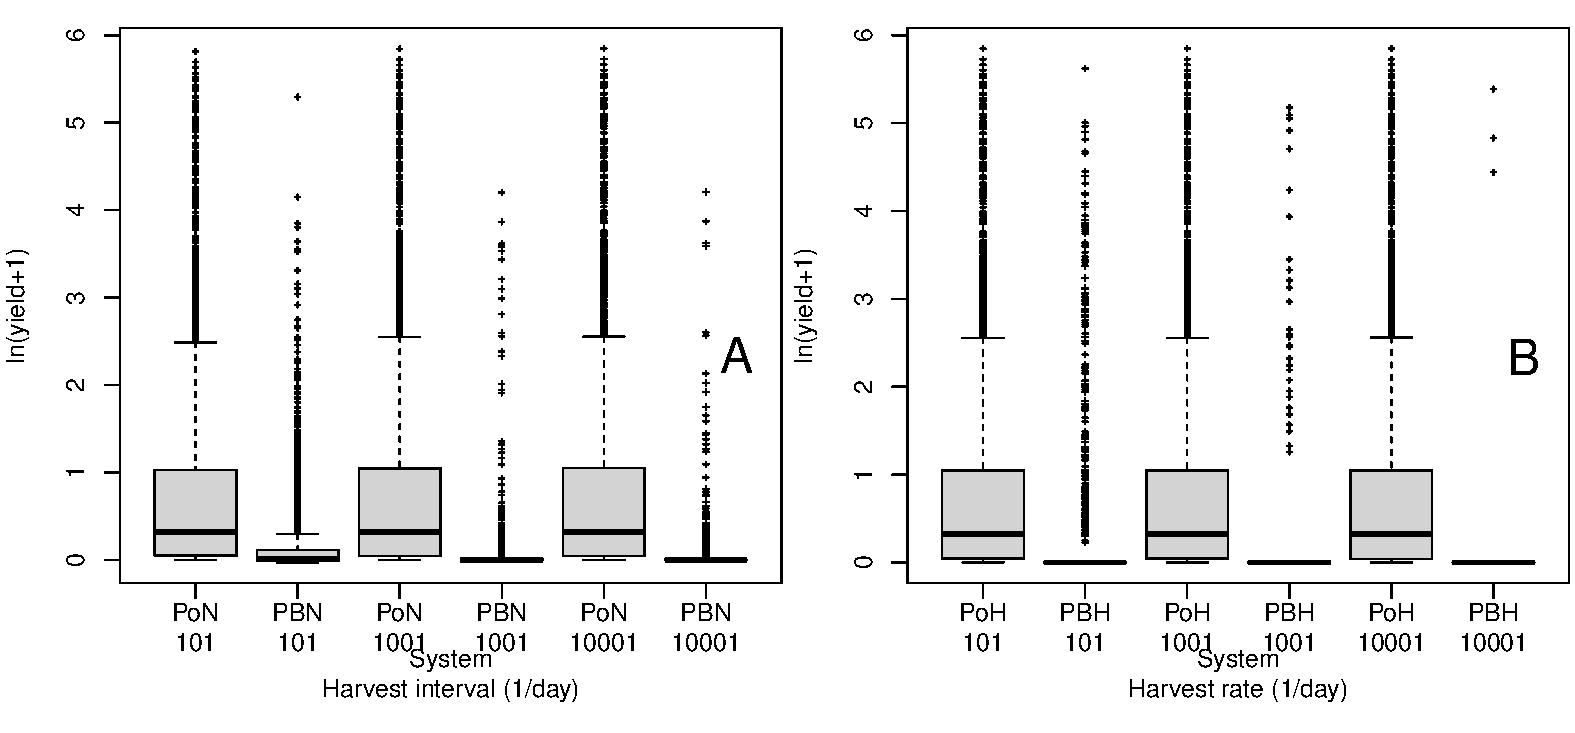
\includegraphics[width=\linewidth]{result/Harvest.pdf}
    \caption[Yield flux distribution by harvest mode]{Log distribution of yield for destructive \textbf{(A)} and continuous \textbf{(B)} harvest modes on selected harvest interval/rates.  \textbf{(A)} Pairwise Wilcox test showed significance (p $\ll$ 0.01) between all except the pair of \PoN\ systems interval 5 and 50 days (p $>$ 0.1).  For \PBN\ systems 0.5 days harvest interval, some systems recorded an initial drop of organic carbon and caused a slight negative yield (none of the drops exhausted the initial organic carbon pool).  The drop recovered in later time with a large variation in yield recovery.  \textbf{(B)} \PoH\ and \PBH\ systems were significantly different (p $\ll$ 0.01).  Significance was also found between \pbs s (p $\ll$ 0.01) but not \phy-only systems (p $>$ 0.1).  Each box represented a sample size of 5500.}
    \label{f:ydByHarv}
\end{figure}

\begin{figure}[H]
    \centering
    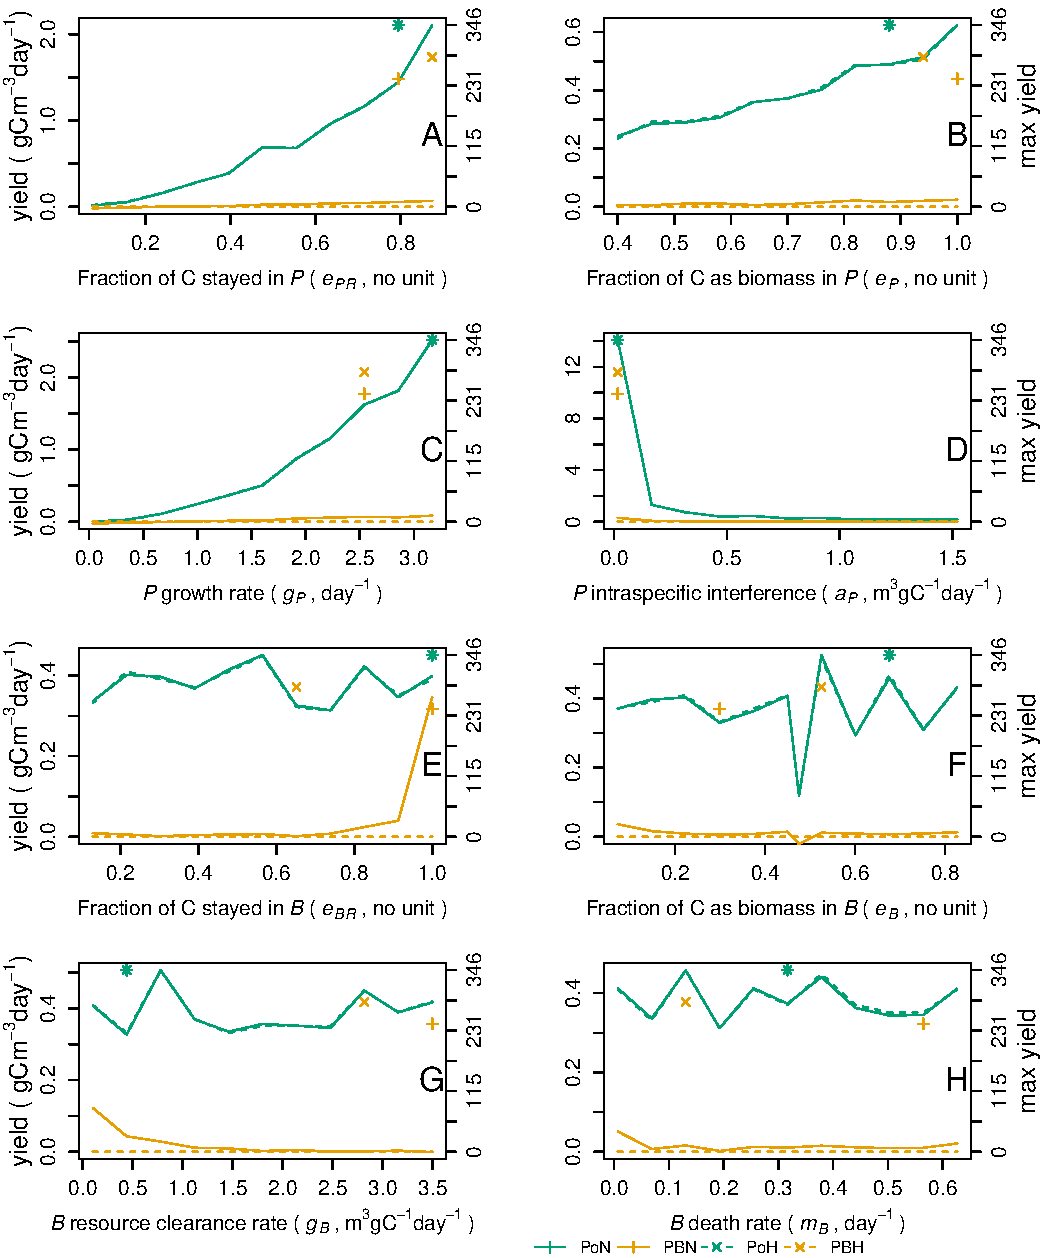
\includegraphics[width=\linewidth]{result/yieldFlux.pdf}
    \caption[Yield flux median in biological parameter space]{Median yield flux (primary axis) and the maximum yield scenario (secondary axis) along respective parameter ranges under a standardised temperature range of \temp.  Each median trend had an LHS sample size of 5500.  Pairwise Wilcox test showed significance (p $\ll$ 0.01) between all systems.  Note that trends between \phy-only and \pbs s had different responses while harvest modes only caused small deviation in median yields.  Also note that in all plots, y-axis range for primary axis was much smaller than the secondary axis.  There were many outliers regardless of the parameter under consideration (Fig.\ref{f:ydByHarv}).}
    \label{f:ydByPara}
\end{figure}

\end{document}